\section{Musée du Louvre}
Louvre, jedno z nejpůsobivějších muzeí na světě, schraňuje více než 350 000 neocenitelných artefaktů. Pevnost, ve které žili králové nechal na muzeum upravit Napoleon Bonaparte.\\
\begin{figure}[h!]
\centering
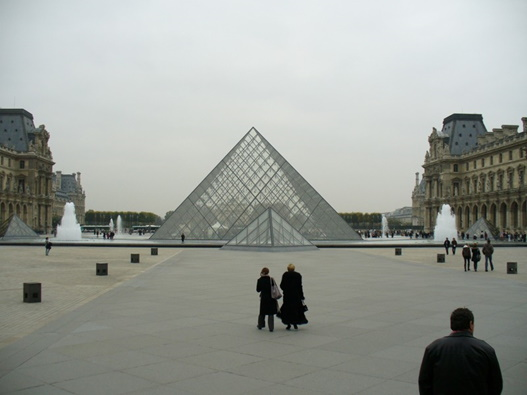
\includegraphics[scale=0.5]{images/obr8L.jpg}
\caption{Musée du Louvre}
\label{lou}
\label{Musée du Louvre}

\end{figure}
\\Hlavní vchod se nachází ve skleněné pyramidě, kterou vidíme na obrázku ~\ref{lou}, ale vejít lze i přes nákupní středisko Carrousel du Louvre v rue de Rivoli. Z haly s pokladnou vybíhají chodby do tří křídel muzea (Sully, Denon a Richelieu), obepínajících několik nádvoří\index{nádvoří}. Díla jsou rozmístěna na čtyřech podlažích a obrazy a sochy jsou uspořádány podle země původu. Uměleckým předmětům, starověkým památkám, grafikám a kresbám jsou věnována samostatná oddělení.\cite{nelson}






\subsection{Francouzské malířství}
Jedinečná kolekce pokrývá období od 14. století do roku 1848 a zahrnuje díla Georgese de La Tour, Jeana-Antoina Watteaua, Jeana-Honorého Fragonarda a dalších umělců.

\subsection{Francouzské sochařství}
K nejcennějším exponátům kolekce se řadí náhrobek\index{náhrobek} Philippa Pota od Antoina Moituriera, Koně z Marly a výtvory Pierra Pugeta na zaskleném nádvoří.

\subsection{Umění starého Egypta}
Nejlepší sbírka staroegyptského umění mimo káhirské muzeum se pyšní sfingou v kryptě, Sedícím písařem ze Sakkáry, rozměrnými sarkofágy, mumifikovanými zvířaty, hrobovými předměty a poutavými sochami zachycujícími každodenní život ve starém Egyptě.

\subsection{Umění starého Řecka}
Úchvatná kolekce umění starého Řecka obsahuje vše od kykladských sošek z 3. tisíciletí před Kristem přes antické řecké sochy z mramoru (asi 5. století př. Kr.) až po poklady z helénistického období (konec 3.-2. století př. Kr.).

\subsection{Starý Orient}
Ohromující sbírka zahrnuje mimo jiné například rekonstrukci paláce asyrského krále a rovněž zákoník\index{zákoník} krále Chammurapiho (18. století př. Kr.), nejstarší právní dokument na světě.

\subsection{Italské malířství}
Francouzská šlechta obdivovala italské umění a shromáždila značnou část zdejší sbírky (1200–1800). Mezi mnoha díly od da Vinciho uvidíte rovněž Monu Lisu, kterou můžeme vidět na obrázku ~\ref{lisa}.

\begin{figure}[h!]
\centering
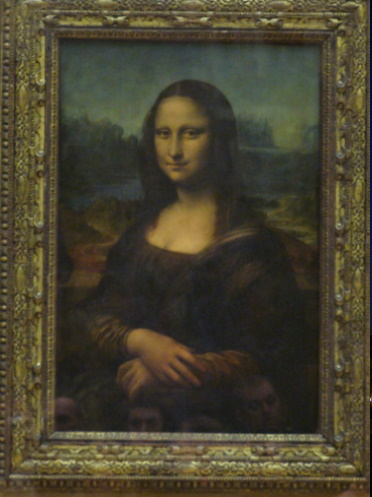
\includegraphics[scale=0.5]{images/obr9M.jpg}
\caption{Musée du Louvre}
\label{lisa}
\end{figure}


\subsection{Italské sochařství}
K nejvýznamnějším exponátům této raně renesanční sbírky náleží madona s dítětem od Donatella, která pochází z poloviny 15. století, a Michalangelovi Otroci.

\subsection{Nizozemské malířství}
Na čestném místě oddělení se vyjímají Rembrantovy práce a také výjevy z interiérů od Vermeera a podobizny od Franse Halse.